\chapter{How to Have the Best Year Ever}

This chapter follows Jim Rohn's seminar talk ``How to Have the Best Year Ever,'' preserved as part of a curated playlist rather than a clean institutional course. Jim Rohn is the original speaker, and the chapter therefore proceeds by practical ratios, repeated acts, and causal chains rather than by formal blackboard derivation. No validated mathematical frame assets survive for this lecture, so every visual reconstruction below is transcript-derived. We shall follow the lecture in its actual order: first the contract of the day, then the autobiographical warrant, then the method of listening, then the five-part life scaffold, and finally the applied domains of goals, money, communication, and resolve.

\section{Investment, Story, and Seminar Terms}

The lecture opens with a joke and then immediately turns serious. The day is not a performance but an investment. Rohn states the hierarchy without hesitation:
\begin{equation}
T > M,
\end{equation}
where \(T\) is time and \(M\) is money. Money may be replaced; time cannot. That is the opening evaluative principle, and the rest of the lecture is an attempt to justify the audience's expenditure of a day.

This opening also explains the role of autobiography. Rohn does not present credentials in institutional form. He presents a life that changed. We move through Idaho farm country, a father still working into old age, one year of college followed by quitting too early, marriage, bills, creditors, embarrassment, and the recognition that one may work hard and still be far behind. The narrative is not decorative. It is the first piece of evidence.

The turning point is Earl Shoaff. Rohn meets a wealthy man who is easy to talk to, philosophically distinctive, and willing to teach. The teaching is concrete: books to read, disciplines to practice, changes in language, changes in personality, changes in how one thinks about one's future. In the lecture's own rhythm, that is where the old life ends and the new life begins. Shoaff's intervention becomes the warrant for everything that follows.

A second autobiographical movement matters as well. After being coached, Rohn discovers that his own story has communicable value. He tells it at a breakfast club, then to management and sales groups, then as a speaking craft. This is important because the lecture will keep insisting that ideas are not inert. They become valuable when translated into practice and then into language that can help others.

By the time he says, in effect, ``Let's go to work,'' the room has already been given a contract, a witness, and a reason to listen.

\section{How to Listen to the Lecture}

Before the lecture offers doctrine, it tells us how it should be received. The sequence matters: sincerity, ideas, inspiration, gratitude, listening, note-taking, and the warning to be students rather than followers. The first distinction is one of the lecture's most important:
\begin{equation}
\mathrm{Sincerity} \neq \mathrm{Truth}.
\end{equation}
A speaker may be sincere and still be wrong. In slightly cleaned notation, the point can be summarized as
\begin{equation}
\mathrm{test}(\mathrm{Sincerity})=\mathrm{Sincerity},
\qquad
\mathrm{test}(\mathrm{Truth})=\mathrm{Truth}.
\end{equation}
This is a cautious reconstruction of the spoken logic, not a board equation. But it captures the lecture exactly. Sincerity proves only that the speaker is sincere; it does not prove that the claim is true.

\subsection{Question \& Answer}

\paragraph{Question.} If sincerity is not truth, how is truth tested?

\paragraph{Answer.} By truth itself, and therefore by reality, by consequences, and later in the lecture by results and numbers. The right response to a sincere speaker is not discipleship but study. We are to process the material, not merely admire the person delivering it.

Rohn then couples ideas with inspiration. He does not allow us to choose one against the other. We need ideas because life can change by a single additional insight. His image is the lock:
\begin{equation}
(n_1,\dots,n_k,n_{k+1}) \Rightarrow \text{lock opens}.
\end{equation}
We may already have five or six numbers in place. The lock still does not open. But that does not mean we need five or six more. We may need one more. A seminar may provide it; a sermon may provide it; a conversation, a lyric, or a line from a film may provide it. The point is not mystical. It is combinatorial and practical: a nearly completed structure may be waiting on one missing term.

At the same time, inspiration remains partly mysterious. Some come, some do not. Some hear, some mock, some are perplexed, some believe. Rohn refuses to waste energy trying to straighten out the entire distribution of human response. His rule is blunt and durable: in every field, some do and some do not. The faces change; the ratios do not change much.

This leads directly to the lecture's next practical commands. Be thankful, because cynicism closes what gratitude opens. Listen well, because much of life will continue outside the room while the lecture is going on. Take good notes, because ideas should outlive the afternoon. And finally, do not become a follower. Become a student. Advice may be taken; orders are not to be accepted. Action must become the product of one's own conclusion.

\section{The Five Major Pieces of the Life Puzzle}

Rohn now announces the first real scaffold of the day: the five major pieces of the life puzzle. He introduces them not as abstract categories but as fundamentals learned in the years immediately after Shoaff entered his life. Their order is explicit:
\begin{equation}
P \to H \to A \to R \to L,
\end{equation}
where \(P\) is philosophy, \(H\) attitude, \(A\) activity, \(R\) results, and \(L\) lifestyle.

This is not a formal theorem. It is a causal ordering of the lecture's own kind. Philosophy comes first because it is the ``set of the sail.'' The winds are shared; the sail-setting is not. One person blames government, taxes, prices, weather, company policy, or circumstances. Another changes the sail. The lecture's insistence is that the second person has begun to understand where leverage really lies.

\paragraph{Transcript-derived schematic.} The following flowchart is a transcript-based reconstruction of the lecture's five-part order.

\begin{figure}
\begin{center}
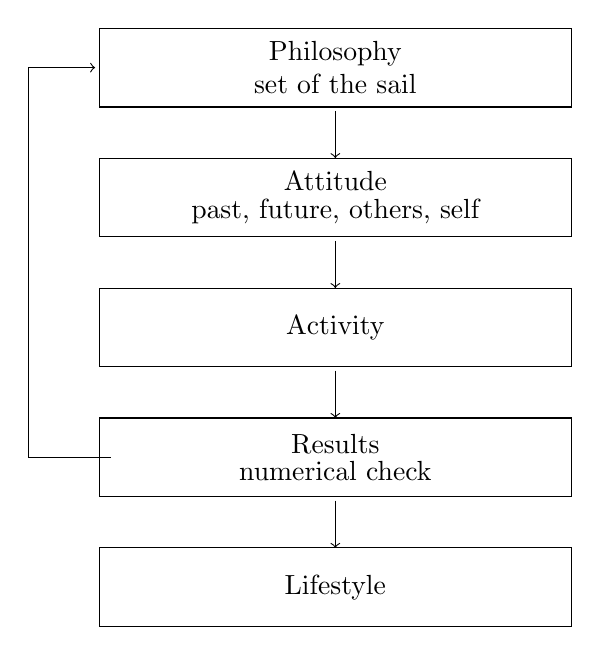
\begin{tikzpicture}[x=1cm,y=1cm]
\draw (0,0) rectangle (6,1);
\node at (3,0.5) {\shortstack{Philosophy\\set of the sail}};

\draw[->] (3,-0.05) -- (3,-0.65);

\draw (0,-1.65) rectangle (6,-0.65);
\node at (3,-1.15) {\shortstack{Attitude\\past, future, others, self}};

\draw[->] (3,-1.70) -- (3,-2.30);

\draw (0,-3.30) rectangle (6,-2.30);
\node at (3,-2.80) {Activity};

\draw[->] (3,-3.35) -- (3,-3.95);

\draw (0,-4.95) rectangle (6,-3.95);
\node at (3,-4.45) {\shortstack{Results\\numerical check}};

\draw[->] (3,-5.00) -- (3,-5.60);

\draw (0,-6.60) rectangle (6,-5.60);
\node at (3,-6.10) {Lifestyle};

\draw[->] (0.15,-4.45) -- (-0.9,-4.45) -- (-0.9,0.50) -- (-0.05,0.50);
\end{tikzpicture}
\end{center}
\end{figure}

The feedback arrow is not spoken as notation, but the lecture clearly relies on it:
\begin{equation}
R \to P_{\text{revised}}.
\end{equation}
Results diagnose philosophy. If the results are poor, philosophy must be amended. If the results are strong, philosophy has at least passed a practical test.

Rohn then makes the argument by way of what cannot be changed. We arrive in a world already stocked with seed, soil, rain, sunshine, seasons, schools, markets, institutions, and the raw possibility of life. These are the givens. If we blame them wholesale, we are blaming all we have to work with. The lecture's metaphysics is therefore severe but liberating: the materials are fixed; the use of them is not.

\subsection{Question \& Answer}

\paragraph{Question.} If the seasons and circumstances do not change, what exactly can we change?

\paragraph{Answer.} We change the inner ordering principle. We change our philosophy first, and then attitude, activity, results, and lifestyle can begin to move with it. This is why the lecture returns to philosophy again and again. It is upstream of the rest.

Attitude is then defined in its stable, recoverable form: attitude toward the past, toward the future, toward other people, and toward oneself. Here the lecture adds a crucial correction. Life change does not begin with inspiration. It begins with education. We do not first whip up feeling and then hope it carries the day. We first learn where we have been mistaken, and only then does feeling acquire a dependable direction.

\section{Errors, Disciplines, and the Numbers of Change}

Once the five-part scaffold has been laid down, the lecture narrows into formulas. These are the strongest quasi-equations in the entire talk:
\begin{align}
\mathrm{Failure} &= \text{a few errors in judgment, repeated every day},\\
\mathrm{Success} &= \text{a few simple disciplines, practiced every day}.
\end{align}
Rohn immediately grounds these formulas in small examples. He does not speak first of grand strategy. He speaks of the apple and the Hershey bar, of walking around the block, of the simple letter not yet written, of the book not yet bought. This is the lecture's major insight into accumulation: the decisive causes are often local, repeatable, and apparently trivial.

\paragraph{Transcript-derived schematic.} The following narrow comparison reconstructs the lecture's central contrast.

\begin{figure}
\begin{center}
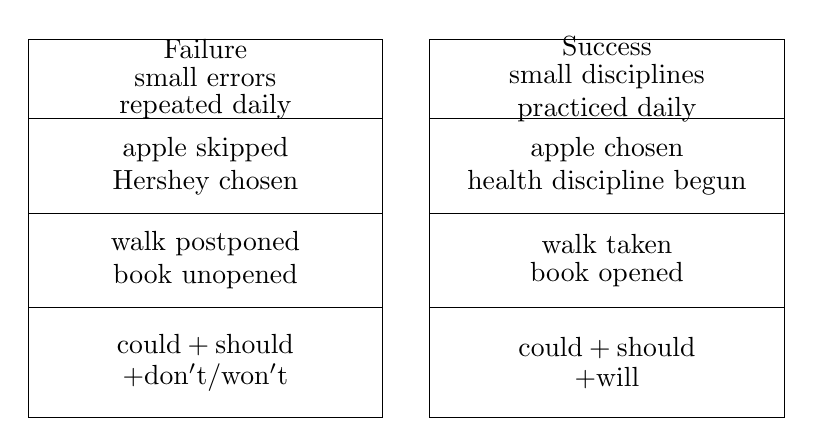
\begin{tikzpicture}[x=1cm,y=1cm]
\draw (0,0) rectangle (4.5,4.8);
\draw (0,3.8) -- (4.5,3.8);
\draw (0,2.6) -- (4.5,2.6);
\draw (0,1.4) -- (4.5,1.4);

\draw (5.1,0) rectangle (9.6,4.8);
\draw (5.1,3.8) -- (9.6,3.8);
\draw (5.1,2.6) -- (9.6,2.6);
\draw (5.1,1.4) -- (9.6,1.4);

\node at (2.25,4.3) {\shortstack{Failure\\small errors\\repeated daily}};
\node at (7.35,4.3) {\shortstack{Success\\small disciplines\\practiced daily}};

\node at (2.25,3.2) {\shortstack{apple skipped\\Hershey chosen}};
\node at (7.35,3.2) {\shortstack{apple chosen\\health discipline begun}};

\node at (2.25,2.0) {\shortstack{walk postponed\\book unopened}};
\node at (7.35,2.0) {\shortstack{walk taken\\book opened}};

\node at (2.25,0.7) {\shortstack{\(\mathrm{could}+\mathrm{should}\)\\\(+\mathrm{don't/won't}\)}};
\node at (7.35,0.7) {\shortstack{\(\mathrm{could}+\mathrm{should}\)\\\(+\mathrm{will}\)}};
\end{tikzpicture}
\end{center}
\end{figure}

The paired practical formulas are then stated directly:
\begin{equation}
\mathrm{could}+\mathrm{should}+\mathrm{don't/won't}\Rightarrow \mathrm{disaster},
\end{equation}
and
\begin{equation}
\mathrm{could}+\mathrm{should}+\mathrm{will}\Rightarrow \mathrm{change}.
\end{equation}
What matters here is not symbolic sophistication but moral direction. The lecture's claim is that disaster is not always dramatic at the beginning. It is often invisible in its first increments. One omitted apple does not immediately produce illness. One missed walk does not immediately produce collapse. The delay is the danger.

\subsection{Question \& Answer}

\paragraph{Question.} If the right act is so simple, why is change still rare?

\paragraph{Answer.} Because what is easy to do is also easy not to do. Simplicity does not remove resistance; it reveals it. Repeated neglect hides inside the fact that the first penalty is small. Repeated discipline hides inside the fact that the first return is also small. Both processes are cumulative.

The lecture now hardens into audit. Results are introduced as the numerical check on philosophy, attitude, and activity. Rohn's teacher asks not for excuses but for counts: money saved, books read, classes taken, calls made, pounds gained. In a compact reconstruction:
\begin{equation}
R=(n_{\text{books}},\,n_{\text{classes}},\,n_{\text{calls}},\,\Delta w,\,s,\dots),
\end{equation}
where the entries stand for the kinds of countable outcomes the lecture explicitly mentions.

\paragraph{Worked example.} Rohn's own sales case is simple enough to display without embellishment. Suppose the weekly target is ten calls:
\begin{align}
n_{\text{calls}}^{\text{target}} &= 10,\\
n_{\text{calls}}^{\text{actual}} &= 1 \quad \text{or} \quad 20.
\end{align}
The lecture's point is that the number already reveals the state of the earlier pieces. A story does not improve the count. The count itself tells us whether philosophy, attitude, and activity are aligned.

This is why the lecture says, bluntly, that results are the name of the game. Life asks for measurable progress in reasonable time. Success is a numbers game because numbers refuse to be flattered.

\section{Personal Development and the Seasonal Cycle}

Having tightened the argument around daily mechanism, the lecture now broadens again. Rohn turns to personal development in the fullest sense. Two spoken principles guide the whole movement. First, it is not what happens that determines the major part of our future; it is what we do about what happens. Second, if we change, everything changes for us. Hence the famous practical injunction: work harder on yourself than on your job.

The lecture's central seasonal model appears here:
\begin{equation}
(\mathcal W,\mathcal{Sp},\mathcal{Su},\mathcal F)
=
(\text{winter},\text{spring},\text{summer},\text{fall}),
\end{equation}
with the associated meanings
\begin{align}
\mathcal W &= \text{adversity},\\
\mathcal{Sp} &= \text{opportunity},\\
\mathcal{Su} &= \text{nourish and protect},\\
\mathcal F &= \text{reap without complaint}.
\end{align}

\paragraph{Transcript-derived schematic.} The following seasonal reconstruction keeps the lecture's tall, narrow logic.

\begin{figure}
\begin{center}
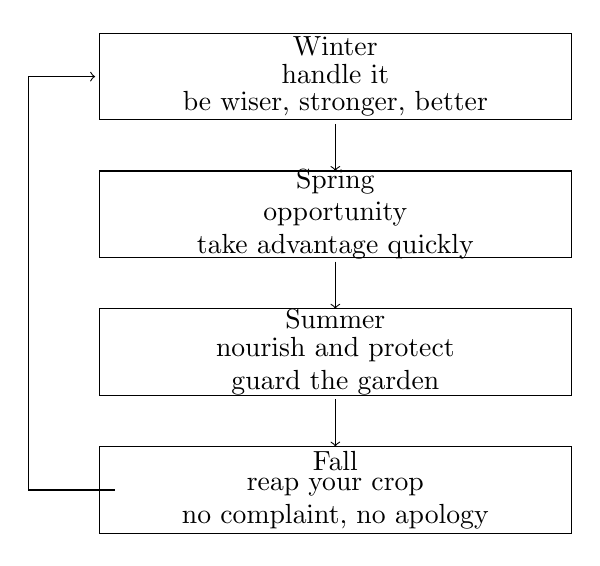
\begin{tikzpicture}[x=1cm,y=1cm]
\draw (0,0) rectangle (6,1.1);
\node at (3,0.55) {\shortstack{Winter\\handle it\\be wiser, stronger, better}};

\draw[->] (3,-0.05) -- (3,-0.65);

\draw (0,-1.75) rectangle (6,-0.65);
\node at (3,-1.20) {\shortstack{Spring\\opportunity\\take advantage quickly}};

\draw[->] (3,-1.80) -- (3,-2.40);

\draw (0,-3.50) rectangle (6,-2.40);
\node at (3,-2.95) {\shortstack{Summer\\nourish and protect\\guard the garden}};

\draw[->] (3,-3.55) -- (3,-4.15);

\draw (0,-5.25) rectangle (6,-4.15);
\node at (3,-4.70) {\shortstack{Fall\\reap your crop\\no complaint, no apology}};

\draw[->] (0.2,-4.70) -- (-0.9,-4.70) -- (-0.9,0.55) -- (-0.05,0.55);
\end{tikzpicture}
\end{center}
\end{figure}

The four lessons are memorable because they are neither sentimental nor grandiose. We cannot abolish winter, so we prepare to meet it. We cannot merely admire spring, so we seize it. We cannot merely celebrate summer growth, so we nourish what is good and defend against what threatens it. We cannot complain about the harvest, so we reap it and take responsibility for it.

This seasonal sequence allows the lecture to widen into the machinery of self-revision. A good library belongs here, because wisdom is one of the instruments by which winter is handled. A journal belongs here, because experience is wasted unless it is gathered. Reflection belongs here because the past must be invested in the future rather than merely survived.

Rohn formulates five abilities for this middle part of the lecture:
\begin{enumerate}
\item the ability to absorb,
\item the ability to respond,
\item the ability to reflect,
\item the ability to act,
\item the ability to share.
\end{enumerate}
The order is important. We first take the day in. We then let it touch feeling. We then go back over it, so that it becomes usable experience. We then act before intention cools. Finally we share, which enlarges our own capacity as well as helping others.

The lecture's ``law of diminishing intent'' belongs exactly here. When the idea is hot and the emotion is strong, that is the time to act. If action is delayed, intention diminishes. Hence the constant practical advice: buy the first book, write the first letter, begin the first walk, do the first push-ups, start the first list. Discipline is how wisdom is captured before it evaporates.

\section{Goals as Designed Future}

Now the lecture turns from general development to designed future. The transition is sharp. Shoaff asks to see Rohn's list of goals. There is no list. Shoaff replies that he can almost guess the bank balance of a man with no goals. This is not merely a motivational flourish. It is the lecture's claim that vagueness about the future has measurable economic consequences in the present.

Goals are then defined as vision. More precisely, the lecture contrasts two states:
\begin{equation}
F_{\text{undesigned}}\Rightarrow \mathrm{apprehension},
\qquad
F_{\text{designed}}\Rightarrow \mathrm{anticipation}.
\end{equation}
If the future is left unshaped, we face it anxiously and take hesitant steps. If it is designed, we face it with anticipation and energy. That is why the lecture warns that if we do not make plans of our own, we usually fall into someone else's plans, and someone else's plans may amount to not much.

A second formula belongs to this same moment:
\begin{equation}
\text{price is easy if the promise is clear}.
\end{equation}
This is one of the lecture's most useful practical statements. The difficulty of discipline is often not in the discipline itself. It is in the dimness of the promised future. When the promise becomes visible, the price becomes payable.

\paragraph{Mechanism.} Rohn's procedure is intentionally plain: decide what you want and write it down. Make a list. What do you want to do, see, be, have, share, support, learn, and be known for? The lecture insists on the written list because unwritten desire remains vapor. Written desire becomes something to review, revise, and pursue.

\paragraph{Anecdote.} The lecture preserves even the comic and petty uses of the list. An early goal-list item is the name of the finance company that humiliated him when he was behind on payments. Later, when he can finally pay the debt off, he turns the repayment into a small private drama and then checks the item off the list. The anecdote matters because it shows that a goal-list need not be lofty in every line. Its function is to turn vague future into concrete sequence.

\subsection{Question \& Answer}

\paragraph{Question.} Why set a millionaire goal if money itself is not the deepest value?

\paragraph{Answer.} Because the major value of the goal lies in what it makes of the person who pursues it. That is Shoaff's correction, and it changes the moral meaning of ambition. The point is not the pile of cash as such; it is the stretch of the self that the goal requires.

The lecture states the principle directly:
\begin{equation}
\text{greatest value in life}\neq \text{what you get},
\qquad
\text{greatest value in life}=\text{what you become}.
\end{equation}
The higher question is therefore not merely ``What am I getting?'' but ``What am I becoming?'' The same applies to work, to income, and to goals themselves.

This account of goals is then given two sharp boundaries. First, do not set goals too low. The easy crowd does not provoke growth. Second, do not compromise what you become in pursuit of what you want. The Judas example, however rhetorically severe, is used for this exact reason: a gain that corrupts the self is not success. Hence the lecture's paired words, ``behold'' and ``beware.'' We are to behold possibility and beware the price of self-betrayal.

\section{Financial Independence, Communication, and Resolve}

\subsection{Financial Independence as Applied Philosophy}

Rohn now turns to economics because economics is easy to count. Here the lecture becomes especially schematic and numerical. The first clarification is decisive:
\begin{equation}
\text{pay} \neq \text{time}.
\end{equation}
Time is necessary, but time as such is not what is bought. The marketplace buys value brought in time. If \(V\) denotes value brought to the marketplace and \(Y\) the resulting income, the lecture's rule can be summarized as
\begin{equation}
V \mapsto 2V \Rightarrow Y \mapsto 2Y
\qquad \text{(in the same time)}.
\end{equation}
That is not a formal economic law. It is a practical rule of leverage. Becoming more valuable is the earnings mechanism.

The dollar-allocation rule is presented with equal bluntness. In transcript-derived cleaned form:
\begin{equation}
1.00=0.70_{\text{spend}}+0.10_{\text{charity}}+0.10_{\text{active capital}}+0.10_{\text{passive capital}}.
\end{equation}
In symbols tied to income \(I\), this becomes
\begin{align}
S &\le 0.70I,\\
(C,K_a,K_p) &= (0.10I,\,0.10I,\,0.10I),
\end{align}
with \(S\) for spending, \(C\) for charity, \(K_a\) for active capital, and \(K_p\) for passive capital. The warning is immediate:
\begin{equation}
O>I \Rightarrow \mathrm{downfall},
\end{equation}
where \(O\) is outgo.

\paragraph{Transcript-derived schematic.} The following visual keeps the lecture's numerical rule narrow and readable.

\begin{figure}
\begin{center}
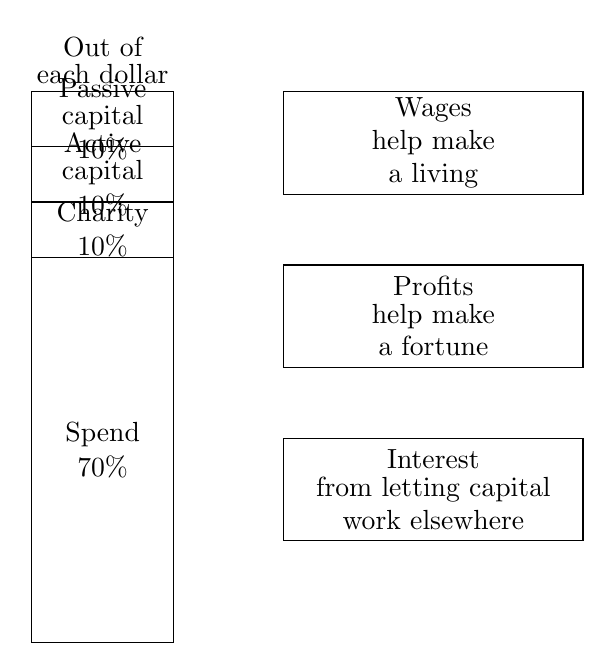
\begin{tikzpicture}[x=1cm,y=1cm]
\draw (0,0) rectangle (1.8,7.0);
\draw (0,0) rectangle (1.8,4.9);
\draw (0,4.9) rectangle (1.8,5.6);
\draw (0,5.6) rectangle (1.8,6.3);
\draw (0,6.3) rectangle (1.8,7.0);

\node at (0.9,7.4) {\shortstack{Out of\\each dollar}};
\node at (0.9,2.45) {\shortstack{Spend\\70\%}};
\node at (0.9,5.25) {\shortstack{Charity\\10\%}};
\node at (0.9,5.95) {\shortstack{Active\\capital\\10\%}};
\node at (0.9,6.65) {\shortstack{Passive\\capital\\10\%}};

\draw (3.2,5.7) rectangle (7.0,7.0);
\node at (5.1,6.35) {\shortstack{Wages\\help make\\a living}};

\draw (3.2,3.5) rectangle (7.0,4.8);
\node at (5.1,4.15) {\shortstack{Profits\\help make\\a fortune}};

\draw (3.2,1.3) rectangle (7.0,2.6);
\node at (5.1,1.95) {\shortstack{Interest\\from letting capital\\work elsewhere}};
\end{tikzpicture}
\end{center}
\end{figure}

\paragraph{Worked example.} If we scale the lecture's dollar into \(I=100\), then the plan reads
\begin{align}
I &= 100,\\
S &\le 70,\\
C &= 10,\qquad K_a=10,\qquad K_p=10.
\end{align}
If instead outgo reaches \(110\), then
\begin{equation}
O-I=10,
\end{equation}
and the lecture's warning applies at once: excess outgo becomes the beginning of downfall.

The lecture then distinguishes three channels of income in plain language:
\begin{itemize}
\item wages help make a living,
\item profits help make a fortune,
\item interest is earned by letting someone else use the capital.
\end{itemize}
Thus, in Rohn's practical sense,
\begin{equation}
\mathrm{profits}>\mathrm{wages},
\end{equation}
and, equally,
\begin{equation}
\mathrm{borrower}\prec \mathrm{lender}.
\end{equation}
The power position is not the spender but the lender.

\paragraph{Attitude.} The lecture is careful not to leave the topic at arithmetic. It immediately adds attitude. Taxes are framed as feeding ``the goose that lays the golden eggs.'' Bills are reframed as opportunities to reduce liabilities and increase assets. We need not enlarge this into a theory of public finance. The lecture's more limited point is that bitterness toward obligation distorts behavior, while a disciplined plan improves it. Hence the repeated maxim: it is not the amount that counts; it is the plan that counts.

\subsection{Communication}

The lecture's communication block is one of its most structured late movements. The stable four-part sequence is:
\begin{enumerate}
\item have something good to say,
\item say it well,
\item read your audience,
\item add intensity with measure.
\end{enumerate}
The block opens from a strong premise: words can work miracles. In the lecture's religious language, words can create light. In its practical meaning, a conversation can move another person from blindness to visibility, from darkness to intelligibility. That is why preparation matters. One cannot speak powerfully from emptiness.

To have something good to say requires at least three things that survive clearly in the transcript: interest, sensitivity, and knowledge. Interest turns frustration into fascination and keeps us teachable. Sensitivity means being touched and moved by other people's situations rather than speaking from self-enclosure. Knowledge means having actually done the reading, the note-taking, the journaling, and the preparation.

To say it well, the lecture emphasizes sincerity, repetition, brevity, and vocabulary. Repetition is the mother of skill. Brevity becomes possible when character carries weight that words no longer need to carry alone. Vocabulary matters because words are a way of seeing and a way of expressing. A thin vocabulary narrows perception, and narrowed perception makes poor judgment more likely.

To read the audience, the lecture offers three channels: read what you see, read what you hear, and read what you feel. That triad is late but stable, and it belongs in these notes exactly because it is practical rather than ornamental.

The whole communication doctrine can be compressed into one cleaned formula:
\begin{equation}
\text{well-chosen words}+\text{measured emotion}\Rightarrow \text{strong communication}.
\end{equation}
The word ``measured'' is essential. The lecture's own image is that one should not shoot a cannon at a rabbit. Emotion gives force, but unmeasured force destroys proportion.

\subsection{Question \& Answer}

\paragraph{Question.} What turns a moral insight into an actual life change rather than another intention?

\paragraph{Answer.} The lecture's answer is sequential. Disgust says ``enough.'' Decision cleans up the list. Desire is triggered and intensified by experience. Resolve says ``I will.'' Then the whole sequence is sustained by the one word Rohn asks us to write down: until.

\subsection{Resolve and the Final Charge}

The lecture's final movement begins by legitimating the negative. There is a time to laugh and a time to cry. Negative is not to be denied; it is to be mastered. Rohn's ant philosophy makes the point vividly: ants never quit, and ants think winter all summer. The summer sky must not deceive us into forgetting the storm.

The positive turn then arrives in a tight sequence:
\begin{equation}
\text{disgust} \to \text{decision} \to \text{desire} \to \text{resolve}.
\end{equation}
Disgust is the day of ``I've had it.'' The lecture illustrates it with the executive woman who asks her husband for ten dollars, hears ``What for?'', and decides she will never ask again. Decision is the clearing of the list. Desire waits for a trigger, and the lecture explicitly lists the possible triggers: a song, a movie, a seminar, a sermon, a book, an enemy, a friend who finally levels with you. Resolve then concentrates the whole movement into the phrase ``I will.''

The lecture's strongest operational word is the next one:
\begin{equation}
\text{resolve} \Rightarrow \text{until}.
\end{equation}
A baby tries to walk until it walks. We read until understanding changes. We listen until it makes sense. We practice until skill appears. The lecture's moral psychology is therefore not built on one surge of feeling but on persistence after feeling has cooled.

The final exhortation then broadens outward. Help people with their lives, not just their jobs. Help them with books, poems, words, mistakes, goals, dreams, and futures. And then the lecture comes to its last reliable sentence: if we work on our gifts, those gifts will make room for us. That line gathers the whole chapter into one image. A disciplined inner development creates outer room.

\section{Summary}

The lecture begins with a contract about time and ends with a claim about gifts. Between those two points it builds a practical chain. Philosophy sets the sail. Attitude follows philosophy. Activity translates both into labor. Results measure whether the prior pieces are sound. Lifestyle is the fashioned form of what those results make possible.

The chapter's strongest formulas all serve this one architecture: time is worth more than money; sincerity is not truth; failure is repeated error; success is repeated discipline; pay is for value rather than hours; designed future turns apprehension into anticipation; outgo beyond income brings downfall; and the final action-engine is disgust, decision, desire, resolve, and until. None of these are offered as abstractions detached from life. Each is introduced through story, resistance, example, and return. That is why the lecture retains its force on the page: it is not merely about getting more. It is about becoming more, and then using that increase to help other lives unfold.